\documentclass{article}
\usepackage{graphicx}
\begin{document}
You're probably familiar with regular word searches, where you're presented with a grid of letters and a word to find.  The word can be in a straight line horizontally, vertically, or diagonally (and perhaps backwards in any of those directions).  For example, here is a grid of letters:

\begin{figure}[!h]
\centering
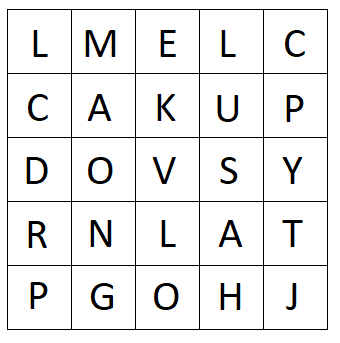
\includegraphics[width=0.25\textwidth]{kinky1.png}
\caption{A word search grid}
\end{figure}

The word ``JAVA'' can be found going from the bottom right corner diagonally upwards.

In a {\em kinky word search\/} the path that spells out the word can have one or more ``kinks'' -- places where the path changes direction.  For example, in the given grid you can spell the word ``PYTHON'' with $3$ kinks (one each at the T, H and  O):

\begin{figure}[!h]
\centering
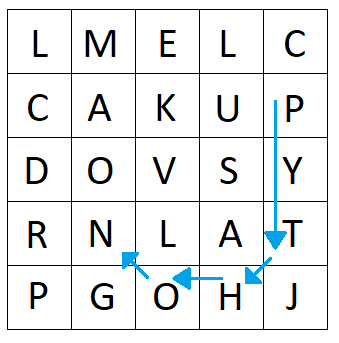
\includegraphics[width=0.25\textwidth]{kinky2.png}
\caption{A kinky spelling of ``PYTHON''}
\end{figure}

Adding kinks allows letters to be reused -- the word ``CPLUSPLUS'' can be found in the upper right corner of the grid (with $5$ kinks).  However you cannot stay on a letter twice in a row, so you cannot spell the word ``HASKELL'' in this grid (though you can find at least $11$ more common programming languages).
Your task is to see if the spelling of a word with a certain number of kinks is possible or not.

\section*{Input}
Input begins with a line containing two positive integers $r$ and $c$ ($r, c \leq 10)$, the number of rows and columns in the grid.  After this are $r$ rows of $c$ uppercase characters.  Letters are separated by a space. After the grid are two lines: The first line is an integer $k$, the number of kinks.  The second line contains an uppercase word to look for, with maximum length $100$.

\section*{Output}

Output either the word {\tt Yes} if it is possible to spell the given word with exactly $k$ kinks on the grid provided, or {\tt No} if it is not.
\end{document}
